% !TEX program = XeLaTeX
% !TEX encoding = UTF-8
\documentclass[UTF8,nofonts]{ctexart}
\setCJKmainfont[BoldFont=FandolSong-Bold.otf,ItalicFont=FandolKai-Regular.otf]{FandolSong-Regular.otf}
\setCJKsansfont[BoldFont=FandolHei-Bold.otf]{FandolHei-Regular.otf}
\setCJKmonofont{FandolFang-Regular.otf}

\usepackage{url}
\usepackage{cancel}
\usepackage{xspace}
\usepackage{graphicx}
\usepackage{multicol}
\usepackage{multirow}
\usepackage{subfig}
\usepackage{amsmath}
\usepackage{amssymb}
\usepackage[a4paper, width=186mm, top=18mm, bottom=18mm, includeheadfoot]{geometry}
\usepackage{booktabs}
\usepackage{array}
\usepackage{verbatim}
\usepackage{caption}
\usepackage{natbib}
\usepackage{booktabs}
\usepackage{float}
\usepackage{pdflscape}
\usepackage{mathtools}
\usepackage[usenames, dvipsnames]{xcolor}
\usepackage{afterpage}
\usepackage{pgf}
\usepackage{tikz}
\usepackage{dirtree}
\usepackage[style=american]{csquotes}
\usepackage{amsfonts}
\usepackage{tikz}
\usepackage{tkz-graph}
\usetikzlibrary{arrows,decorations.pathmorphing,automata,positioning,backgrounds,fit,shapes.symbols,chains,intersections}
\usepackage{scrextend}
\addtokomafont{labelinglabel}{\sffamily}

\newtheorem{definition}{Definition}[section]
\newtheorem{theorem}{Theorem}[section]
\newtheorem{lemma}{Lemma}
\newtheorem{proof}{Proof} [section]

\usepackage[toc, page, title, titletoc, header]{appendix}
\usepackage{marginnote}
\usepackage{tablefootnote}
\usepackage{tabu}

\renewcommand\abstractname{摘要}

\usepackage{perpage} %the perpage package
\MakePerPage{footnote} %the perpage package command

\usetikzlibrary{shapes.geometric}%
\usepackage{color}
%\usepackage[pages=some, placement=top]{background}
\usepackage{eso-pic}
\usepackage[final]{pdfpages}

%\includepdf[pages=1]{cover}
\hyphenpenalty=750

\title{\textbf{Vite:}\textbf{高性能异步去中心化应用平台}}
\author{
  刘春明\\
  \texttt{charles@vite.org}\\
  \and
  王东\\
  \texttt{daniel@loopring.org}\\
  \and
  伍鸣\\
  \texttt{woo@vite.org}\\
 }
\date{}
\makeatletter
\def\CTEX@section@format{\Large\bfseries}
\makeatother

\makeatletter
\newenvironment{tablehere}
 {\def\@captype{table}}
 {}
 
\newenvironment{figurehere}
 {\def\@captype{figure}}
 {}
\makeatother

\begin{document}

\maketitle

\begin{abstract}
Vite是一个通用的去中心化应用平台,在兼顾安全性的同时,满足了工业级应用对高吞吐、低延迟和扩展性的要求。Vite采用DAG账本结构,账本中的交易按账户分组。Vite中的快照链结构,可以弥补账本自身防篡改能力的不足。通过分层共识算法HDPoS,将交易的写入和确认解耦,并保障系统的高性能和扩展性。Vite的虚拟机部分兼容EVM,智能合约语言在Solidity基础上进行了适当扩展,提供了更为强大的描述能力。另外,在Vite设计中,一个重要改进是采用了基于消息驱动的异步架构,智能合约之间通过消息传递信息,从而极大提高了系统的吞吐率和扩展性。Vite除了内置原生代币之外,还支持用户发行自己的数字资产,同时提供了跨链价值传输以及基于路印协议\cite{loopring}的资产互换功能。Vite通过配额来实现资源配置,低频用户无需支付交易手续费。另外,Vite还支持定时调度、命名服务、合约升级、区块裁剪等功能。
\end{abstract}

\begin{multicols}{2}

\section{简介}
\subsection{定义}

一个通用去中心化应用(dApp)平台,可以支持一组智能合约,每个智能合约都是一个拥有独立状态以及不同操作逻辑的交易状态机,它们之间可以通过消息传递的方式进行通信。

从整体上,这个系统是一个交易状态机。系统的状态$\boldsymbol{s}\in\boldsymbol{S}$也称为世界状态,是由每一个独立账户的状态构成的。一个能够引起账户状态改变的事件称为交易。更形式化的定义如下:

\begin{definition}[交易状态机] \label{def:fsm}
一个交易状态机是一个四元组: $(\boldsymbol{T},\boldsymbol{S},\boldsymbol{g},\boldsymbol{{\delta}})$,其中,$\boldsymbol{T}$是交易的集合,$\boldsymbol{S}$是状态的集合,$\boldsymbol{g} \in \boldsymbol{S}$为初始状态,也称为“创世块”,$\boldsymbol{{\delta}:\boldsymbol{S}\times\boldsymbol{T}\rightarrow\boldsymbol{S}}$是状态转移函数。
\end{definition}

这种交易状态机的语义是一个离散迁移系统,定义如下:
\begin{definition}[交易状态机的语义] \label{def:semantics}
一个交易状态机$(\boldsymbol{T},\boldsymbol{S},\boldsymbol{g},\boldsymbol{{\delta}})$的语义是一个离散迁移系统: $(\boldsymbol{S},\boldsymbol{g},\boldsymbol{\rightarrow})$,其中,$\boldsymbol{\rightarrow} \in \boldsymbol{S}\times\boldsymbol{S}$,表示迁移关系。
\end{definition}

同时,去中心化应用平台是一个分布式系统,具有最终一致性。通过某种共识算法,节点间可以就最终的状态达成一致。在现实场景中,智能合约的状态中保存的是一个去中心化应用的全部数据,体积比较大,无法在节点间传输。因此,节点间需要通过传递一组交易,来达成最终状态的一致。我们将这样的一组交易组织成某种特定的数据结构,通常称之为账本。

\begin{definition}[账本] \label{def:ledger}
账本是由一组交易构成的,具有递归构造的抽象数据类型,定义如下:
$$
\left\{\begin{matrix}
l = \Gamma(T_{t})\\ 
l = l_{1} + l_{2}
\end{matrix}\right.
$$
其中,$T_{t} \in 2^{T}$,表示一组交易, $\Gamma \in 2^{T} \rightarrow L$,表示通过一组交易构造一个账本的函数,$L$是账本的集合,$\boldsymbol{+}: L \times L \rightarrow L$,表示将两个子账本合并成一个账本的操作。
\end{definition}

需要注意的是,在此类系统中,账本通常用来表示一组交易,而不是一个状态。在比特币\cite{nakamoto2008bitcoin}和以太坊\cite{wood2014ethereum}中,账本是一个区块链结构,其中交易是全局有序的。修改账本中的一个交易,需要重新构造账本中的一个子账本,从而提高了篡改交易的成本。

根据同一组交易,可以构造出不同的有效账本,但它们所表示的交易顺序不同,因此可能会导致系统进入不同的状态。当这种情况发生时,通常称账本发生了“分叉”。
\begin{definition}[分叉] \label{def:fork}
设$T_{t},{T_{t}}' \in 2^{T}$,$T_{t} \subseteq {T_{t}}'$。若$l=\Gamma_{1}(T_{t})$,${l}'= \Gamma_{2}({T_{t}}')$,且不满足$l \preceq {l}'$,则称$l$和${l}'$是分叉账本。$\preceq$表示前缀关系。
\end{definition}

根据交易状态机的语义,我们可以很容易的证明,从一个初始状态开始,如果账本不分叉,则每个节点最终会进入相同的状态。那么,如果接收到分叉的账本,就一定进入不同的状态吗?这取决于账本中交易的内在逻辑,以及账本如何组织交易之间的偏序。现实中,经常会出现一些满足交换律的交易,却因为账本设计的问题,频繁的引起分叉。当系统从一个初始状态出发,接收两个分叉的账本,最终进入同一状态,我们称这两个账本为伪分叉账本。

\begin{definition}[伪分叉] \label{def:falsefork}
有初始状态$s_{0} \in S$,账本$l_{1},l_{2} \in L$,$s_{0}\overset{l_{1}}{\rightarrow}s_{1}, s_{0}\overset{l_{2}}{\rightarrow}s_{2}$。若$l_{1} \neq l_{2}$,且$s_{1}=s_{2}$,则称这两个账本$l_{1} ,l_{2}$为伪分叉(false fork)账本。
\end{definition}

一个设计良好的账本,应该尽量降低伪分叉发生的概率。

当分叉发生时,每个节点都需要从多个分叉的账本中选择一个,为确保状态的一致性,这些节点需要采用同一个确定的算法完成选择,这个算法称为共识算法。

\begin{definition}[共识算法] \label{def:consensus}
共识算法是一个函数,它接收一个账本的集合,返回其中唯一一个账本:
$$\Phi: 2^{L} \rightarrow L$$
\end{definition}

共识算法是系统设计的一个重要内容,一个好的共识算法应该具有较高的收敛速度(convergence speed),减少共识在不同分叉间摇摆,并对恶意攻击具有较高的防范能力。

\subsection{当前进展}
以太坊\cite{buterin2017ethereum}率先实现了这样一个系统。
在以太坊的设计中,世界状态的定义是:$S = \Sigma^{A}$,是由每个账户$a \in A$与该账户的状态$\sigma_{a} \in \Sigma$构成的映射。因此,以太坊的状态机中任何一个状态都是全局的,这表示一个节点在每个时刻都可以获取任何一个账户的状态。

以太坊的状态转移函数$\delta$,是由一组程序代码来定义的,每组代码被称为一个智能合约。以太坊定义了一个图灵完备的虚拟机,称为EVM,运行在其上的指令集称为EVM代码。用户可以通过一种语法类似于javascript的程序语言Solidity来开发智能合约,并编译成EVM代码,部署到以太坊上\cite{dannen2017introducing}。一旦智能合约部署成功,就相当于定义了该合约账户$a$收到一个交易后的状态转移函数$\delta_{a}$。
EVM目前在此类平台中被广泛使用,但它也存在一些问题。例如,缺少库函数支持,安全性问题突出等。

以太坊的账本结构是区块链\cite{nakamoto2008bitcoin},区块链由区块构成,每一个区块中包含一组交易的列表,后一个区块引用前一个区块的hash,构成一个链状结构。
\begin{equation}
\Gamma(\lbrace t_{1}, t_{2},...\vert t_{1}, t_{2},... \in T \rbrace) = (..., (t_{1}, t_{2},...)) 
\end{equation}
这个结构的最大好处是有效的防止交易被篡改,但由于它维护的是所有交易的全序,任何两个交易交换顺序,都会生成一个新账本,也造成这种结构具有较高的分叉概率。事实上,在这个定义下,交易状态机的状态空间被看作一棵树:初始状态是根节点,不同的交易顺序代表不同的路径,叶子节点是最终状态。现实的情况下,大量叶子节点的状态是相同的,这就造成了大量的伪分叉。

以太坊的共识算法$\Phi$称为PoW,该算法率先在比特币协议中提出\cite{nakamoto2008bitcoin}。PoW算法依赖于某个易于验证但难于求解的数学问题,例如,根据一个hash函数$h:N \rightarrow N$,求解$x$,使$h(T+x) \geq d$,$d$是一个给定的数,称为难度,T是区块中包含的交易列表的二进制表示。在区块链的每个区块中,都会包含这类问题的一个解。将全部区块的难度加起来,就是一个区块链账本的总难度:
\begin{equation}
D(l) = D(\sum_{i} l_{i}) = \sum_{i} D(l_{i})
\end{equation}

因此,在从分叉中选择正确账本的时候,只要选择总难度最高的分叉即可:
\begin{equation}
 \Phi (l_{1}, l_{2}, ..., l_{n}) = l_{m} \text{ where } m = \arg\max_{i \in 1..n}(D(l_{i}))
\end{equation}

PoW共识算法具有较好的安全性,迄今为止在比特币和以太坊中运行得很好。但这个算法有两个主要问题,第一是求解数学难题需要消耗大量计算资源,造成能源浪费;第二是该算法收敛速度较慢,因而影响了系统整体的吞吐率。目前,以太坊整体的TPS只有15左右,完全无法满足去中心化应用的需求。

\subsection{改进方向}
在以太坊诞生之后,以太社区和其他一些同类项目开始从不同方向对系统加以改进。从系统的抽象模型来看,可以改进的方向主要包括以下几个:
\begin{itemize}
	\item 改进系统状态$\boldsymbol{S}$	
	\item 改进状态迁移函数$\boldsymbol{\delta}$	
	\item 改进账本结构$\boldsymbol{\Gamma}$
	\item 改进共识算法$\boldsymbol{\Phi}$
\end{itemize}

\subsubsection{改进系统状态}
对系统状态的主要改进思路是将全局的世界状态局部化,每个节点不再关心全部交易和状态转移,只维护整个状态机的一个子集。这样集合$S$和集合$T$的势都大为缩减,从而提高了系统扩展性。此类系统包括:Cosmos\cite{cosmos},Aelf\cite{aelf},PChain等。

从本质上讲,此类基于侧链的方案牺牲了状态的全局性,以换取系统的扩展性。这使得每个运行在其上的dApp的去中心化程度都被削弱——一个智能合约的交易历史不再被全网每一个节点保存,而只被一部分节点保存。
除此之外,跨合约交互也会成为此类系统的瓶颈。例如,Cosmos中,不同的Zone交互,需要通过一个共同的链Hub来完成\cite{cosmos}。

\subsubsection{改进状态迁移函数}
一些项目立足于改进EVM,提供更为丰富的智能合约编程语言。例如,RChain	定义了一种基于$\pi$演算的智能合约语言Rholang;NEO中的智能合约称为NeoContract,可以用Java,C\# 等主流编程语言开发;EOS使用C/C++来编程。

\subsubsection{改进账本结构}
账本结构的改进方向是构造等价类,将多个交易全局有序的线性账本规约为一个只记录部分偏序关系的非线性账本,这种非线性账本结构是一个DAG(有向无环图)。目前,Byteball\cite{byteball},IOTA\cite{iota},Nano\cite{nano}等项目基于DAG的账本结构实现了加密货币功能。也有一些项目在尝试利用DAG实现智能合约,但迄今为止在这个方向上的改进还在探索中。

\subsubsection{改进共识算法}
共识算法的改进大部分是为了提高系统的吞吐率,主要方向是抑制伪分叉的产生。下面我们讨论伪分叉与哪些因素有关。

\begin{center}
\begin{figurehere}
\includegraphics[width=.7\linewidth]{image/falsefork.png}
\caption{伪分叉}
\end{figurehere}
\end{center}

如图所示,$L$是针对某个交易集合所有可能的分叉账本的集合,$S$是以不同顺序执行这一组交易,所能到达的状态的集合。根据定义 \ref{def:fork},映射$f: L \rightarrow S$是一个满射;而根据定义 \ref{def:falsefork},这个映射不是单射。下面我们来计算伪分叉的概率:

假设共有$C$个用户有权生产账本,$M = \vert L \vert$,$N = \vert S \vert$,$M_{i} = \vert L_{i} \vert$, 其中,$L_{i} = \lbrace l \vert f(l) = s_{i}, s_{i} \in S \rbrace$。
则伪分叉概率为:
\begin{equation}
P_{ff} = \sum_{i=1}^{N}\left ( \frac{M_{i}}{M} \right )^{C} - \frac{1}{M^{C-1}}
\end{equation}

从这个公式可以看出,为了降低伪分叉概率,可以有两种途径:
\begin{itemize}
	\item 在账本集合$L$上建立等价关系,对其划分等价类,构造分叉更少的账本
	\item 限制有权生产账本的用户,从而减少$C$
\end{itemize}

第一种途径是Vite设计的重要方向,后文将详细论述;第二种途径现在已被多种算法所采用。在PoW算法中,任何用户都有权生产区块;而PoS算法将生产区块的权力限制在那些拥有系统权益的用户中;DPoS算法\cite{dpos}将有权生产区块的用户进一步限制在一组代理节点范围内。
	
目前,通过改良共识算法,已经产生出一些比较有影响力的项目。例如,Cardano采用了一种PoS算法,称为Ouroboros,文献\cite{bernardo2017ouroboros}对该算法相关性质给出了严格证明;EOS\cite{eos}采用的BFT-DPOS算法,是DPoS算法的一个变种,通过快速生产区块,提高系统的吞吐率;Qtum\cite{dai2017smart}的共识算法本质上也是一种PoS算法;RChain\cite{rchain}采用的Casper算法也是PoS算法的一种。

还有一些其他项目在共识算法的改进上提出了自己的方案。NEO\cite{neo}采用了一种BFT算法,称为dBFT;Cosmos\cite{cosmos}采用了一种称为Tendermint\cite{tendermint}的算法。

\section{账本}
\subsection{概述}
账本的作用主要是为了确定交易之间的顺序,交易的顺序会影响以下两个方面:
\begin{itemize}
	\item \textbf{状态一致性:} 由于系统的状态不是一个CRDT(Conflict-free replicated data types)\cite{crdt},因此,交易不都是可交换的,不同的交易执行顺序可能会导致系统进入不同的状态。
	\item \textbf{hash有效性:} 账本中,交易会被打包成区块,区块中包含互相引用的hash。交易的先后顺序会影响账本中hash引用的连通性。这种影响的范围越大,篡改交易的成本就越大。这是因为,改变任何一个交易,都必须重建所有直接或间接引用该交易的区块的hash。
\end{itemize}

而账本的设计也有两个主要目标:

\begin{center}
\begin{figurehere}
\includegraphics[width=.7\linewidth]{image/ledger-merge.png}
\caption{账本合并}
\end{figurehere}
\end{center}

\begin{itemize}
	\item \textbf{降低伪分叉率:} 如前文讨论,降低伪分叉率可以通过建立等价类,尽量将导致系统进入同一状态的一组账本合并成一个账本来实现。如上图,根据伪分叉率公式可以算得,左图的账本伪分叉率$P_{ff}=\left (  \frac{3}{5} \right )^{C} + \left (  \frac{2}{5} \right )^{C} - \frac{1}{5^{C-1}}$;而合并账本空间后,右图的伪分叉率为${P_{ff}}'=\left (  \frac{2}{3} \right )^{C} + \left (  \frac{1}{3} \right )^{C} - \frac{1}{3^{C-1}}$。可知当$C > 1$,${P_{ff}}' < P_{ff}$。也就是说,我们应尽量减小账本中交易之间的偏序关系,允许更多的交易之间的顺序可交换。
	\item \textbf{防篡改:} 当账本$l$中一个交易$t$被修改,账本的两个子账本$l = l_{1} + l_{2}$中,子账本$l_{1}$不受影响,而子账本$l_{2}$中的hash引用需要重建,以构成一个新的有效账本${l}' = l_{1} + {l_{2}}'$。受影响的子账本$l_{2} = \Gamma(T_{2}),T_{2} = \lbrace x \vert x \in T, x > t \rbrace $。由此可见,想提高篡改交易的成本,需要在账本中尽量多的维护交易之间的偏序关系,以扩大篡改的影响范围$\vert T_{2} \vert$。
\end{itemize}

\begin{center}
\begin{figurehere}
\includegraphics[width=\linewidth]{image/ledger-compare.png}
\caption{账本结构比较}
\end{figurehere}
\end{center}

显然,以上两个目标是互相矛盾的,在设计账本结构时必须作出必要的权衡取舍。由于账本维护的是交易之间的偏序,因此它本质上是一个偏序集(poset)\cite{poset},如果用哈斯图(Hasse diagram)\cite{hasse}来表示,在拓扑上就是一个DAG。

上图对比了几种常见的账本结构,靠近左侧的账本维护更少的偏序关系,哈斯图显得比较扁平,具有更低的伪分叉率;靠近右侧的账本维护更多的偏序关系,哈斯图比较细长,具有更高的防篡改特性。

图中,最左侧的是一种中心化系统中常见的基于集合的结构,没有任何防篡改特性;最右侧则是典型的区块链账本,具有最好的防篡改特性;而介于二者中间的是两种DAG账本,左侧的是Nano采用的block-lattice账本\cite{nano},右侧是IOTA采用的tangle账本\cite{iota}。从特性上看,block-lattice维护了更少的偏序关系,更适合作为高性能去中心化应用平台的账本结构。但由于它的防篡改特性较差,会产生安全隐患,因此,迄今为止,除了Nano采用了该结构之外,还没有其他项目采用。

为了追求高性能,Vite采用该账本结构。同时,通过引入一种额外的链式结构Snapshot Chain,并且改进了共识算法,成功的弥补了block-lattice安全性方面的不足,后文将详细论述这两个改进。

\subsection{前提约束}
首先,我们来看一下采用这种账本结构对状态机模型的前置要求。这种结构本质上是将整个状态机看作是一组独立的状态机的组合,每个账户对应一个独立的状态机,每个交易只影响一个账户的状态。在账本,对所有交易按账户分组,并把同一账户的交易组织成一条链。因此,我们对Vite中的状态$S$和交易$T$做出如下限制:

\begin{definition}[交易的单自由度约束]
系统状态$s \in S$,是由每个账户的状态$s_{i}$构成的向量$s=(s_{1}, s_{2},...,s_{n})$。对于$\forall t_{i} \in T$,执行交易$t_{i}$后,系统状态发生如下转移:$({s_{1}}',..., {s_{i}}',...,{s_{n}}') = \sigma(t_{i}, (s_{1},..., s_{i},...,s_{n}))$,需满足:${s_{j}}'=s_{j} , j \neq i$。该约束称为交易的单自由度约束。
\end{definition}

直观上,一个单自由度的交易只会改变一个账户的状态,不会影响系统中其他账户的状态。在状态空间向量所在的多维空间中,执行一次交易,系统状态只会沿平行于某个坐标轴的方向移动。请注意,这个定义要比比特币、以太坊等模型中的交易定义更为严格,比特币中的一个交易,会改变发送者和接收者两个账户的状态;以太坊则可能通过消息调用,改变两个以上的账户的状态。

在这个约束条件下,交易之间的关系得以简化。任何两个交易,要么是正交的,要么是平行的。这为依照账户对交易进行分组提供了条件。下面举一个例子来说明:

\begin{center}
\begin{figurehere}
\includegraphics[width=.8\linewidth]{image/tx-deg-of-free.png}
\caption{单自由度交易和中间状态}
\end{figurehere}
\end{center}

如上图所示,假设Alice和Bob各有10元钱,系统的初始状态为$s_{0} = (10, 10)$。当Alice想给Bob转账2元时,在比特币和以太坊的模型中,可以通过一个交易${t}'$,使系统直接进入最终状态:$s_{0} \overset{{t}'}{\rightarrow}{s}'$。

而在Vite的定义中,交易${t}'$同时改变了Alice和Bob两个账户的状态,不符合单自由度的原则。因此,这个交易必须被拆分成两笔交易:

1) 表示Alice转出2元的交易$t_{1}$

2) 表示Bob转入2元的交易$t_{2}$。

这样,从初始状态到达最终状态${s}'$可以有两条不同的路径$s_{0} \overset{t_{1}}{\rightarrow} s_{1} \overset{t_{2}}{\rightarrow} {s}'$和$s_{0} \overset{t_{2}}{\rightarrow} s_{2} \overset{t_{1}}{\rightarrow} {s}'$。这两条路径分别通过中间状态$s_{1}$和$s_{2}$,这两个中间状态是最终状态${s}'$在两个账户上维度的投影。也就是说,如果只关心其中某一个账户的状态,只需要执行该账户对应的所有交易,而不需要执行其他账户的交易。

下面我们来定义如何将以太坊中的交易,拆分成Vite所要求的单自由度交易:
\begin{definition}[交易分解]
将一个自由度大于1的交易拆分成一组单自由度交易的过程,称为交易分解。一笔转账交易可以拆分成一个出账交易和一个入账交易;一个合约调用交易可以拆分成一个合约请求交易和一个合约响应交易;每个合约内部的消息调用,可以拆分成一个合约请求交易和一个合约响应交易。
\end{definition}

这样,账本中就有两种不同类型的交易,它们被称为“交易对”:
\begin{definition}[交易对]
一个出账交易或合约请求交易,统称为“请求交易”;一个入账交易或合约响应交易,统称为“响应交易”。一个请求交易和一个对应的响应交易,称为交易对。发起请求交易$t$的账户,记作$A(t)$;对应的响应交易记作:$\widetilde{t}$,该交易对应的账户,记作$A(\widetilde{t})$。
\end{definition}

根据以上定义,我们可以得出Vite中,任何两个交易之间可能存在的关系:
\begin{definition}[交易的关系]
对于两个交易$t_{1}$和$t_{2}$,可能存在如下关系:

\textbf{正交}:若$A(t_{1}) \neq A(t_{2})$,则称两个交易正交,记作$t_{1} \perp t_{2}$;

\textbf{平行}:若$A(t_{1}) = A(t_{2})$,则称两个交易平行,记作$t_{1} \parallel t_{2}$;

\textbf{因果}:若$t_{2} = \widetilde{t_{1}}$,则称两个交易具有因果关系,记作$t_{1} \rhd t_{2}$,或者$t_{2} \lhd t_{1}$。
\end{definition}

\subsection{账本定义}
定义一个账本,就是定义一个偏序集。首先,我们来定义Vite中,交易之间的偏序关系:
\begin{definition}[交易的偏序]
我们用二元关系$<$来表示两个交易的偏序关系,有:

一个响应交易,必须排在一个对应的请求交易之后:$t_{1} < t_{2} \Leftrightarrow t_{1} \rhd t_{2}$;

一个账户的所有交易,必须严格全局有序:$\forall t_{1} \parallel t_{2}$,必有:$t_{1} < t_{2}$,或$t_{2} < t_{1}$。
\end{definition}

由于建立在交易集合$T$上的偏序关系$<$满足:
\begin{itemize}
	\item 非自反性(irreflexive):$\forall t \in T$,不存在$t < t$;
	\item 传递性(transitive):$\forall t_{1},t_{2},t_{3} \in T$,若$t_{1}<t_{2},t_{2}<t_{3}$,则有$t_{1}<t_{3}$;
	\item 非对称性(asymmetric):$\forall t_{1},t_{2} \in T$,若$t_{1}<t_{2}$,则不存在$t_{2}<t_{1}$
\end{itemize}

这样,我们就可以用严格偏序集的方式来定义Vite的账本:

\begin{definition}[Vite账本]
Vite账本是给定的交易集合$T$,以及偏序关系$<$,所构成的严格偏序集。
\end{definition}

\begin{center}
\begin{figurehere}
\includegraphics[width=.7\linewidth]{image/ledger.png}
\caption{Vite账本及交易之间的依赖关系}
\end{figurehere}
\end{center}

一个严格偏序集,可以对应到一个DAG结构。如上图所示,圆圈表示交易,箭头表示交易之间的依赖关系,$a \rightarrow b$表示$a$依赖于$b$。

上面所定义的Vite账本,结构类似于block-lattice。交易分为请求交易和响应交易两种,每个交易对应一个单独的区块,每个账户$A_{i}$对应一条链,一个交易对中,响应交易引用其对应的请求交易的哈希。

\section{快照链}
\subsection{交易确认}
当账本发生分叉时,共识结果可能会在两个分叉账本间摇摆。例如,基于区块链结构的系统,如果节点接收到一个更长的分叉链,就会选择这个新分叉作为共识结果,而原分叉将被废弃,原分叉上的交易也会被回滚。在此类系统中,交易被回滚是一个非常严重的事件,将会导致双花(double spend)。试想,一个商家接收到一笔付款,提供了商品或服务,之后这笔付款又被撤回,商家可能会因此面临损失。因此,用户在收到一笔付款交易时,需要等待系统对这笔交易进行“确认”,以确保这笔交易被回滚的概率足够低。

\begin{definition}[交易确认]
当一个交易被回滚的概率小于一个给定的阈值$\epsilon$时,称该交易为已确认(confirmed)。
$P_{r}(t) < \epsilon \Leftrightarrow t \text{ is } \boldsymbol{confirmed}$。
\end{definition}

交易的确认是一个非常容易被混淆的概念,因为一个交易是否被确认实际上取决于隐含的置信度$1-\epsilon$。一个售卖钻石的商家和一个售卖咖啡的商家,在被双花攻击的时候,所蒙受的损失是不同的。因此,前者需要对交易设置更小的$\epsilon$。这也是比特币中确认数的本质。在比特币中,确认数表示一个交易在区块链中的深度,确认数越大,交易被回滚的概率越低\cite{nakamoto2008bitcoin}。因此,商家可以通过设置等待多少确认数,间接设定确认的置信度。

交易被回滚的概率随时间而降低,是由于账本结构中存在hash引用关系。如前文所述,当账本的设计具有较好的防篡改特性时,回滚一个交易需要重构该交易所在区块的所有后继区块。随着新的交易被不断加入账本,某个交易的后继节点也越来越多,因此,被篡改的概率也随之下降。

而block-lattice结构中,由于交易是按账户分组的,一个交易只会附加到其所属账户的账户链末端,大部分其他账户产生的交易不会自动成为该交易的后继节点。因此,采用这个结构必须合理的设计共识算法,以避免双花的隐患。

Nano采用了一个基于投票的共识算法\cite{nano},由一组用户选择的代表节点对交易进行签名,每个代表节点有一个权重,当某个交易获得的签名累计起来有足够多的权重时,就认为该交易被确认。这个算法有以下几个问题:

首先,如果需要更高的确认置信度,则需要提高投票权重的阈值,如果没有足够多的代表节点在线,就无法保证收敛速度,有可能一个用户永远也搜集不到确认一个交易所必需的票数;

其次,交易被回滚的概率不随时间递减。这是因为任何时候,推翻一个历史投票的结果,所付出的成本都是一样的。

最后,历史的投票结果并没有被持久化到账本中,只保存在节点的本地存储中。当一个节点从其他节点获取账本时,没有办法可靠的量化一个历史交易被回滚的概率。

从本质上,投票的机制是一个偏中心化的解决方案。我们可以把投票结果看作是对账本状态的一个快照,这个快照会分布式的保存在网络中各个节点的本地存储中。为了拥有和区块链同样的防篡改能力,我们可以将这些快照也组织成链式结构,这就是Vite设计的核心之一——快照链\cite{snapshotchain}。

\subsection{快照链的定义}
快照链是Vite中最重要的存储结构,它的主要作用是维护Vite账本的共识。首先我们给出快照链的定义:
\begin{definition}[快照块和快照链]
一个快照块存储一个Vite账本的状态快照,状态包括:账户的余额、合约状态的Merkle root,每个账户链中最后一个块的hash。快照链是由快照块组成的链式结构,后一个快照块引用前一个快照块的hash。
\end{definition}

一个用户账户的状态包含余额和账户链最后一个块的hash;一个合约账户的状态,除了包含以上两个字段之外,还包含该账户合约状态的Merkle root hash。账户的状态的结构如下:

\begin{verbatim}
  struct AccountState {
    // 账户余额
    map<uint32, uint256> balances;
    // 合约状态的Merkle root
    optional uint256 storageRoot;
    // 账户链最后一个交易的hash
    uint256 lastTransaction;
  }
\end{verbatim}

快照块的结构定义如下:
\begin{verbatim}
  struct SnapshotBlock {
    // 前一个块的hash    
    uint256 prevHash;
    // 快照信息
    map<address, AccountState> snapshot;
    // 签名
    uint256 signature;
  }
\end{verbatim}

为了同时支持多种代币,Vite的账户状态中,记录余额信息的结构不是一个\texttt{uint256},而是一个代币id到余额的映射。

快照链中第一个快照块称为“创世快照”,保存的是账本中创世块的快照。

\begin{center}
\begin{figurehere}

\includegraphics[width=.7\linewidth]{image/snapshotchain.png}
\caption{快照链}
\end{figurehere}
\end{center}

由于快照链中每个快照块都对应于Vite账本的唯一分叉,因此,在快照块不发生分叉的情况下,通过快照块,可以确定Vite账本的共识结果。

\subsection{快照链与交易确认}

引入了快照链之后,block-lattice结构天然的安全性缺陷就得到了弥补。攻击者想生成一个双花交易,除了要重建Vite账本中的hash引用之外,还需要重建快照链中,首次快照该交易的快照块之后的所有区块,并且需要产生一条更长的快照链。这样,攻击成本将大大提高。

在Vite中,交易的确认机制类似于比特币,定义如下:

\begin{definition}[Vite交易确认]
在Vite中,一个交易被快照链所快照,则成为该交易被确认。第一次快照该交易的快照块的深度,称为交易的确认数。
\end{definition}

在这个定义下,快照链每增长一个区块,此前所有已确认交易的确认数都增加1,双花攻击成功的概率随着快照链的不断增加而逐渐下降。这样,用户就可以根据具体的场景,通过等待不同的确认数,来定制所需的确认置信度。

快照链本身依赖一个共识算法,如果快照链发生分叉,则选取\textbf{最长的}分叉作为合法分叉。当快照链切换到新的分叉时,原有快照信息会被回滚,相当于原来对账本达成的共识被推翻,由新的共识结果取代。因此,快照链是整个系统安全性的基石,需要非常认真的对待。

\subsection{压缩存储}
由于快照链中每一个快照块都需要保存所有账户的状态,耗费的存储空间非常大,因此需要对快照链进行压缩。

\begin{center}
\begin{figurehere}
\includegraphics[width=.7\linewidth]{image/compact-snapshot.png}
\caption{压缩前的快照}
\end{figurehere}
\end{center}

压缩快照链存储空间的基本思路是利用增量存储:一个快照块只保存相比于前一个快照块发生变化的数据。如果一个账户在两个快照之间没有发生任何交易,则后一个快照块不保存该账户的数据。

要恢复快照信息,可以从前向后依次遍历快照块,将每一个快照块中的数据覆盖到当前的数据上即可。

\begin{center}
\begin{figurehere}
\centering
\tikzstyle{block} = [draw, fill=blue!20, rectangle, 
    minimum height=3em, minimum width=6em]
\tikzstyle{sum} = [draw, fill=blue!20, circle, node distance=1cm]
\tikzstyle{input} = [coordinate]
\tikzstyle{output} = [coordinate]
\tikzstyle{pinstyle} = [pin edge={to-,thin,black}]

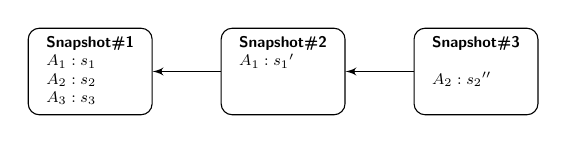
\begin{tikzpicture}[
    auto, 
    node distance=2cm,
    >=latex',
    font=\bfseries\footnotesize\sffamily,
    snapshot/.style={
		scale=0.7,
		rectangle,
		rounded corners,
		draw=black, 
		text centered,
%		text width=5cm,
		minimum height=12mm,
		fill=white
	},
	label/.style={
		scale=0.7
	}
  ]
    % We start by placing the blocks

  \node [snapshot] (snapshot2) 
 {%
 \begin{tabular}{l}
  \textbf{Snapshot\#2}\\
  $A_{1}: {s_{1}}'$\\
  \\
  \\
 \end{tabular}
 };
 
  \node [snapshot, xshift=-3.5cm] (snapshot1) 
 {%
 \begin{tabular}{l}
  \textbf{Snapshot\#1}\\
  $A_{1}: s_{1}$\\
  $A_{2}: s_{2}$\\
  $A_{3}: s_{3}$
 \end{tabular}
 };
 
 
  \node [snapshot, xshift=3.5cm] (snapshot3) 
 {%
 \begin{tabular}{l}
  \textbf{Snapshot\#3}\\
  \\
  $A_{2}: {s_{2}}''$\\
  \\
 \end{tabular}
 };
 
 \draw [draw,->] (snapshot2) -- (snapshot1);
 \draw [draw,->] (snapshot3) -- (snapshot2);

\end{tikzpicture}

\caption{压缩后的快照}
\label{fig:compact-snapshot}
\end{figurehere}
\end{center}

由于每个快照只保存在快照时刻每个账户最后的状态,不关心中间状态,无论在两个快照块之间,一个账户产生了多少交易,在快照中也只保存一份数据。因此,一个快照块最多占用$S * A$个字节。其中,$S = \text{sizeof}(s_{i})$,为每个账户状态占用的字节数,$A$是系统总账户数。如果活跃账户与总账户数的平均比例是$a$,则压缩率为$1-a$。

\section{共识}
\subsection{设计目标}
在设计共识协议时,我们需要充分考虑以下因素:
\begin{itemize}
	\item \textbf{性能}。Vite的首要设计目标是快速,为确保系统具有高吞吐、低延迟的性能表现,我们需要采用具有更高收敛速度的共识算法。
	\item \textbf{扩展性}。Vite是一个公共平台,向所有去中心化应用开放,因此,扩展性也是一个重要的考量因素。
	\item \textbf{安全性}。虽然Vite的设计理念不是追求极致的安全性,但仍然需要确保足够的安全性底线,有效防范各类攻击。
\end{itemize}

对比现存的一些共识算法,PoW的安全性更好,在恶意节点的算力低于50\%的情况下可以确保达成共识。但PoW的收敛速度较慢,无法满足性能要求;
PoS及其变种算法去掉了求解数学难题的步骤,提高了收敛速度和单次攻击成本,降低了能源消耗。但PoS的扩展性仍然较差,而且Nothing at Stake问题\cite{problems}较难解决;
BFT系列算法在安全性和性能方面有较好表现,但其扩展性是一个问题,通常比较适合于私有链或联盟链;
DPoS\cite{dpos}系列算法通过限制生成区块的权限,有效降低了伪分叉率,在性能和扩展性方面表现良好。相应的,DPoS在安全性方面稍有牺牲,需要保证恶意节点数不超过1/3\cite{dpos2}。

综合来看,DPoS算法在性能、扩展性方面有比较明显的优势,因此,我们选择DPoS作为Vite共识协议的基础,并在其基础上进行适当扩展,通过分层共识协议和异步模型,进一步提高平台的整体性能。

\subsection{分层共识}
Vite的共识协议称为HDPoS(Hierarchical Delegated Proof of Stake)。基本思想是对共识函数$\Phi$进行函数分解(functional decomposition):
\begin{equation}
\begin{split}
\Phi(l_1,l_2,\dots,l_n) = \Psi(\Lambda_1(l_1,l_2,\dots,l_n), \\
\Lambda_2(l_1,l_2,\dots,l_n),\dots \\
\Lambda_m(l_1,l_2,\dots,l_n))
\end{split}
\end{equation}

其中,$\Lambda_i: 2^L \rightarrow L$,称为局部共识函数,返回的结果称为局部共识;$\Psi: 2^L \rightarrow L$,称为全局共识函数,它从一组候选的局部共识中选取一个唯一结果,作为最终的共识结果。

这样拆分之后,整个系统的共识变成了两个独立的过程:
\begin{labeling}{alligator}
\item [局部共识] 生产用户账户或合约账户中的请求交易和响应交易对应的区块,并写入账本;
\item [全局共识] 对账本中的数据进行快照,生产快照块。如果账本有分叉,则选择其中一个。
\end{labeling}

\subsection{区块生产权和共识组}
那么,谁有权生产账本中的交易区块和快照链中的快照块,采用什么共识算法达成共识呢?

由于Vite的账本结构是按账户不同组织成多条账户链的,我们可以方便的按账户的维度来限定账本中区块的生产权,再加上快照块的生产权归属于单独的一组用户。这样,我们就可以将若干条账户链或快照链归入一个共识组,在共识组内部,用统一的方式来生产区块并达成共识。

\begin{definition}[共识组]
共识组是一个元组$(L, U, \Phi, P)$,描述了账本的一部分或快照链的共识机制。其中,$L \in A \vert \{ A_s \}$,表示账本中属于该共识组的一条或若干条账户链,或者是快照链;$U$表示拥有$L$指定的链上区块生产权的用户;$\Phi$指定该共识组的共识算法;$P$指定共识算法的参数。
\end{definition}

在这样的定义下,用户可以根据需要,灵活的设置共识组,并选择不同的共识参数。下面我们对不同的共识组加以详细说明:

\subsubsection{快照共识组}
快照链所在的共识组称为快照共识组,这是Vite中最重要的一个共识组。快照共识组的共识算法$\Phi$对应分层模型中的$\Psi$,采用DPoS算法。由参数$P$指定代理节点数和出块间隔。

例如,我们可以指定快照共识组有25个代理节点,以1秒为间隔生产快照块。这样可以保证交易的确认速度足够快,一个交易达到10次确认最多需要等待10秒。

\subsubsection{私有共识组}
私有共识组只适用于账本中交易区块的生产,属于私有共识组的账户链,区块只能由账户的私钥拥有者来生产。默认情况下所有用户账户都属于私有共识组。

私有共识组的最大好处是降低分叉概率。因为只有一个用户有权生产区块,发生分叉的唯一可能是用户主动发起双花攻击,或程序发生错误。

私有共识组的缺点是用户节点必须在线,才能打包交易。这对合约账户来说不太适合,一旦合约拥有者的节点失效,没有其他节点可以代替它生产合约的响应交易,相当于降低了dApp的服务可用性。

\subsubsection{委托共识组}
在委托共识组中,由一组指定的代理节点,通过DPoS算法,代替用户打包账户链上的交易。无论是用户账户还是合约账户,都可以加入委托共识组。用户可以设置一组单独的代理节点,建立一个新的委托共识组。Vite中还有一个默认的委托共识组,来帮助所有未单独建立委托共识组的账户打包交易,这个共识组也称为\textbf{公共共识组}。

委托共识组适合于大部分合约账户,因为合约账户的交易大部分都是合约响应交易,相比于用户账户的收款交易,需要更高的可用性和更低的延迟。

\subsection{共识的优先级}\label{sec:consensus-prio}
在Vite协议中,全局共识的优先级高于局部共识。当局部共识发生分叉的时候,以全局共识选择的结果为准。也就是说,一旦全局共识选定局部共识的一个分叉作为最终结果,即使未来账本中某个账户链出现更长的分叉,也不会使全局共识结果回滚。

在实现跨链协议的时候,这个问题需要格外注意。由于某个目标链可能发生回滚,映射该链的中继合约对应的账户链也需要随之回滚。这个时候,如果中继链的局部共识已经被全局共识采纳,是无法完成回滚的,可能会导致中继合约和目标链的数据不一致。

避免这个问题的方法是在共识组参数$P$中设置一个\textit{delay}参数,指定快照共识组在局部共识完成后\textit{delay}个区块之后,才开始进行快照。这样将大大降低中继合约不一致的概率,但也无法完全避免。在中继合约的代码逻辑中,还需要对目标链回滚的情况做单独处理。

\subsection{异步模型}
为了进一步提高系统吞吐,我们需要在共识机制上支持更完善的异步模型。

一个交易的生命周期包括:交易发起、交易写入、交易确认。为了提高系统的性能,我们需要将这三个步骤设计成异步模式。这是因为在不同的时刻,用户发起交易的数量是不同的,而系统处理交易写入和确认交易的速度相对固定。异步模式有利于削平波峰波谷,从而提高系统的整体吞吐能力。

比特币和以太坊等系统的异步模型比较简单:将所有用户发起的交易放入一个未确认交易池中,当矿工将其打包到一个区块中,该交易同时完成了写入和确认,当区块链继续增长时,该交易最终到达预设的确认置信度。

这个异步模型存在两个问题:
\begin{itemize}
	\item 交易在未确认状态下没有持久化到账本。未确认的交易是不稳定的,没有参与共识,也无法防止交易重复发送;
	\item 交易的写入和确认之间没有异步机制。交易只有在确认时才写入账本,写入速度受制于确认速度。
\end{itemize}

Vite协议建立了更完善的异步模型:首先,将交易拆分成基于“请求-响应”模式的交易对,无论是转账还是合约调用,当一个请求交易被写入账本,则代表该交易被成功发起。另外,交易被写入账本和确认也是异步的。交易可以先被写入Vite的DAG账本中,不会被确认过程阻塞。交易的确认通过快照链来完成,快照的动作也是异步进行的。

这是一个典型的生产者-消费者模型,在交易的生命周期中,无论上游的生产速率如何变动,下游都可以以恒定的速率消化待处理的交易,从而充分利用平台资源,提高了系统的吞吐。

\section{虚拟机}
\subsection{EVM兼容性}
当前以太坊已经拥有大量开发者,也有不少基于Solidity和EVM开发的智能合约投入应用。因此,我们决定在Vite的虚拟机上提供EVM兼容性,大部分EVM指令集可以在Vite中保持原有语义。但由于Vite的账本结构及交易定义与以太坊不同,一些EVM指令的语义需要重新定义,例如获取区块信息的一组指令。详细的语义差异可以参考附录\ref{app:evm-instruction-set}。

其中,差异最大的是消息调用的语义,下面我们来详细讨论。

\subsection{事件驱动}
在以太坊的协议中,一个交易或消息,可能会影响多个账户的状态。例如一个合约调用交易,可能会通过消息调用,使多个合约账户状态同时发生变化。这些状态变化要么同时发生,要么就一个都不发生。因此,以太坊中的交易实际上是一种满足 ACID (Atomicity, Consistency, Isolation, Durability)\cite{Haerder:1983:PTD:289.291}特性的刚性事务,这也是以太坊缺乏扩展性的一个重要原因。

基于扩展性及性能考虑,Vite采用了满足BASE(Basically Available, Soft state, Eventual consistency)\cite{Pritchett:2008:BAA:1394127.1394128}语义的最终一致性方案。具体来说,我们将Vite设计成一个事件驱动的架构(Event-Driven Architecture, EDA)\cite{eda}。每个智能合约被看作是一个独立的服务,合约之间可以通过消息通信,但不共享任何状态。

因此,我们需要在Vite的EVM中,取消跨合约进行同步函数调用的语义,只允许合约间通过消息通信。受影响的EVM指令主要是\textbf{CALL},和\textbf{STATICCALL}。在Vite EVM中,这两条指令不会立即执行,也不会返回调用的结果,只会生成一个请求交易写入账本。因此,这个指令在Vite中不再有函数调用的语义,而是向一个账户发送消息。

\subsection{智能合约语言}
以太坊提供了一种图灵完备的编程语言Solidity,用于开发智能合约。为了支持异步语义,我们对Solidity进行了扩展,定义了一组用于消息通信的语法。扩展之后的Solidity称为Solidity++。

Solidity++将支持Solidity的大部分语法,但不再支持合约外的函数调用。开发者可以通过\emph{message}关键字来定义消息,并通过\emph{on}关键字定义消息处理器(Message Handler),从而实现跨合约通信功能。

下面举一个例子,合约A需要调用合约B中的add()方法,根据返回值更新自己的状态。在Solidity中,可以通过函数调用的方式来实现,代码如下:

\begin{verbatim}
pragma solidity ^0.4.0;

contract B {
    function add(uint a, uint b) returns
    (uint ret) { 
        return a + b;
    }
}

contract A {
    uint total;    
   
    function invoker(address addr, uint a,
    uint b) {
        // message call to A.add()
        uint sum = B(addr).add(a, b);
        // use the return value
        if (sum > 10) {
            total += sum;
        }
    }
}
\end{verbatim}

而在Solidity++中,函数调用代码\texttt{uint sum = B(addr).add(a, b);}不再有效,取而代之的是,合约A和合约B通过彼此发送消息来进行异步通信。代码如下:

\begin{verbatim}
pragma solidity++ ^0.1.0;

contract B {
    message Add(uint a, uint b);
    message Sum(uint sum);
    
    Add.on {
        // read message
        uint a = msg.data.a;
        uint b = msg.data.b;
        address sender = msg.sender;
        // do things 
        uint sum = a + b;
        // send message to return result
        send(sender, Sum(sum));
    }
}

contract A {
    uint total;    
   
    function invoker(address addr, uint a,
    uint b) {
        // message call to B
        send(addr, Add(a, b))        
        // you can do anything after sending
        // a message other than using the 
        // return value
    }
    Sum.on {
        // get return data from message
        uint sum = msg.data.sum;
        // use the return data
        if (sum > 10) {
            total += sum;
        }
    }
}
\end{verbatim}

在代码第一行,通过\texttt{pragma solidity++ \^0.1.0;}定义了源代码是用Solidity++编写的,将不能直接使用Solidity编译器编译,以避免编译出的EVM字节码有不符合预期的语义。Vite会提供一个专门的编译器,用于编译Solidity++。这个编译器是部分向前兼容的:如果Solidity代码中没有与Vite语义冲突的部分,将可以直接通过编译,否则会报错。例如,本地函数调用、向其他账户转账等语法将保持兼容;获取跨合约函数调用的返回值,以及货币单位\texttt{ether}等将无法通过编译。

合约A中,当\texttt{invoker}函数被调用时,会向合约B发送\texttt{Add}消息,这个过程是异步的,结果不会当场返回。因此,需要在A中通过\texttt{on}关键字定义一个消息处理器,用于接收返回结果并更新状态。

合约B中会监听消息\texttt{Add},在处理完成后,通过向消息\texttt{Add}的发送者发送一个\texttt{Sum}消息来返回结果。

Solidity++中的消息会被编译成\textbf{CALL}指令,并生成一个请求交易加入账本。在Vite中账本充当了合约之间异步通信的消息中间件,可以确保消息可靠存储并防止重复。同一个合约发往某个合约的多个消息,可以保证FIFO(First In First Out);不同合约向同一个合约发送的消息并不保证FIFO。

需要注意的是,Solidity中的事件(Event)和Solidity++中的消息不是同一个概念。事件是通过EVM日志,间接向前端发送通知的。

\subsection{标准库}
在以太坊上开发智能合约的开发者,经常被Solidity缺乏标准库的问题所困扰。例如,路印协议中的环路验证必须在链外执行,其中一个重要原因就是Solidity没有提供浮点运算功能,尤其是求浮点数的n次方根\cite{loopring}。

在EVM中,可以通过\textbf{DELEGATECALL}指令来调用一个预先部署的合约,实现库函数的功能。以太坊也提供了几个预编译合约(Precompiled Contract),主要是几个Hash运算。但这些功能都太过简单,无法满足复杂的应用需求。

因此,我们将在Solidity++中,提供一系列标准库,例如:字符串处理、浮点运算、基本数学运算、容器、排序等。

基于性能考虑,这些标准库将以本地扩展(Native Extension)的方式实现,将大部分运算内置到Vite本地代码中,只在EVM代码中通过\textbf{DELEGATECALL}指令来完成方法的调用。

标准库可以根据需要不断扩展,但由于整个系统的状态机模型是确定性的,因此无法提供类似于随机数之类的功能。同以太坊类似,我们可以通过快照链的hash来模拟伪随机数。

\subsection{燃料}
燃料(Gas)在以太坊中主要有两个作用,一是量化EVM代码执行所消耗的计算资源和存储资源,二是确保EVM代码停机。根据可计算性理论,图灵机上的停机问题(Halting Problem)是一个不可计算问题\cite{haltingproblems}。也就是说,无法通过分析EVM代码来判断一个智能合约能否在有限次执行后停止。

因此,Vite中也保留了EVM中的燃料计算。不过在Vite中,没有燃料价格(Gas Price)这个概念,用户不是通过支付手续费的方式来购买一次交易所需的燃料,而是通过一种基于配额的模型,来获取计算资源。配额的计算将在后文“经济模型”章节详细讨论。

\section{经济模型}
\subsection{原生代币}
为了量化平台计算和存储资源,激励节点运行,Vite内置了一种原生代币ViteToken。代币的基本单位为\textit{vite},最小单位为\textit{attov},$1 \: vite = 10^{18} \: attov$。

快照链是影响Vite平台安全性和性能的关键,为激励节点参与交易验证,Vite协议对快照块的生产设置了锻造奖励。

与此相反,当用户发行新代币、部署合约、注册VNS域名\footnote{参见  \textit{\ref{sec:vns} 命名服务}}、获取资源配额时,都需要消耗或者抵押ViteToken。

这两种因素共同作用,有利于优化系统资源的配置。

\subsection{资源配置}
由于Vite是一个通用的dApp平台,部署在其上的智能合约功能各不相同,每一个不同的智能合约,对吞吐和延迟的需求也不同。即使是同一个智能合约,在不同阶段对性能的要求也不同。

在以太坊的设计中,每一个交易在发起时需要指定一个gas price,从而与其他交易竞争写入账本的机会。这是一个典型的竞价模型,原则上可以通过价格有效调控供给和需求的平衡。但由于用户在出价之前,很难量化当前的供需情况,也无法预测其他竞争者的出价,很容易发生市场失灵(market failure)。而且,每次出价所竞争的资源都是针对一个交易的,没有一个按账户维度对资源进行合理配置的协议。

\subsubsection{配额计算}
我们在Vite中采用了一个基于配额的资源配置协议,这个协议允许用户通过三种方式来获取更高的资源配额:
\begin{itemize}
\item 在发起交易时计算一个PoW;
\item 在账户中抵押一定数量的\textit{vite};
\item 一次性销毁少量\textit{vite}。
\end{itemize}

具体的配额可以通过下面的公式来计算:

\begin{equation}
Q = Q_{m} \cdot \left ( \frac{2}{1+exp\left ( -\rho \times \xi^{\top} \right )} - 1  \right )
\end{equation}

其中,$Q_{m}$为一个常数,代表单个账户配额的上限,和系统总吞吐以及账户总数相关。$\xi=(\xi_{d}, \xi_{s}, \xi_{f})$是一个向量,代表用户为获取资源所付出的代价:$\xi_{d}$是用户在生成一个交易时计算出的PoW难度,$\xi_{s}$是账户中抵押的\textit{vite}余额,$\xi_{f}$是用户愿意为提高配额所支付的一次性费用。需要注意的是,$\xi_{f}$不同于手续费,这部分\textit{vite}将直接销毁,而不是支付给矿工。

式中,向量$\rho=(\rho_{d}, \rho_{s}, \rho_{f})$表示通过这三种获取配额方式的权重,
也就是说,销毁1 \: \textit{vite}所换取的配额,相当于抵押$\rho_{s} / \rho_{f}$ \: \textit{vite}。

从这个公式可以看出,如果用户既不抵押\textit{vite}也不支付一次性费用,就必须计算一个PoW,否则将没有配额发起交易,这样可以有效防止粉尘攻击,保护系统资源不被滥用。同时,这个公式是一个Logistic函数,用户获取较低的配额相对比较容易,从而降低了低频使用者的门槛;而高频用户为了获取较高的配额,则需要投入大量资源,他们所支付的额外成本将增加平台全体用户的权益。

\subsubsection{资源量化}
由于快照链相当于一个全局时钟,我们可以利用它准确的量化一个账户的资源使用情况。在每个交易中,必须引用一个快照块的哈希,将快照块的高度作为该交易的时间戳。因此可以根据两个交易时间戳的差,来判断这两个交易之间是否间隔足够长的时间。

\begin{center}
\begin{figurehere}
\includegraphics[width=.8\linewidth]{image/snapshotchain-clock.png}
\caption{快照链作为全局时钟}
\end{figurehere}
\end{center}

如上图所示,账户$A$在2个时间间隔内产生了4个交易,而账户$B$只产生了2个交易。因此,这段时间内$A$的平均TPS是$B$的2倍。如果只是转账交易,量化账户的平均TPS就足够了。而对于智能合约来说,每个交易所消耗的资源都不同,因此需要累计每个交易的燃料,来计算一段时间内的平均资源消耗。一个账户链上高度为n的交易,其最近$k$笔交易的平均资源消耗为:

\begin{equation}
Cost_{k}(T_n) = \frac{k \cdot \sum_{i=n-k+1}^{n}gas_{i}}{timestamp_{n} - timestamp_{n-k+1} + 1} 
\end{equation}

其中,对于一个交易$T_n$,$timestamp_n$为交易的时间戳,也就是它所引用的快照块的高度;$gas_n$为该交易消耗的燃料。

节点在验证一个交易时,会判断配额是否满足条件$Cost(T) \leq Q$,如果不满足,该笔交易会被拒绝。在这种情况下,用户需要重新打包一个交易,通过支付一次性费用等方式增加配额,或者等待一段时间,在交易中引用一个高度更大的快照块。

\subsubsection{配额租赁}
如果用户持有较多\textit{vite}资产,但不需要使用那么多的资源配额,可以选择将自己的配额租赁给其他用户。

Vite系统支持一种特殊的交易类型,用于转移一个账户资源配额的使用权。在该交易中可以指定一个抵押的\textit{vite}数量,一个受让人地址,以及一个租赁时长。一旦交易被确认,与该抵押代币数量对应的资源配额将计入受让人的账户。一旦超过租赁时长,配额将重新计入转让人账户。租赁时长单位为秒,系统将换算成快照块的高度差,因此可能会有一定误差。

用户通过租赁可以获取租金收益,Vite系统只提供配额转让的交易,租金的定价和支付可以通过一个第三方智能合约来实现。

\subsection{资产发行}
除了原生代币ViteToken之外,Vite还支持用户发行自己的代币。发行代币可以通过一种特殊的交易——“铸币交易”(Mint Transaction)来完成。铸币交易的目标地址是0,在交易的\textit{data}字段中,指定代币的参数,格式如下:
\begin{verbatim}
Mint: {
    name: "MyToken",
   	totalSupply: 99999999900000000000000000,
   	decimals: 18,
   	owner: "0xa3c1f4...fa",
    symbol: "MYT"
}
\end{verbatim}

一旦该请求被网络接受,铸币交易所包含的\textit{vite}将作为铸币费从发起者账户扣除。系统会记录新代币的信息,为其分配一个\textit{token\_id}。新生成的代币全部余额都会被加入到\textit{owner}的地址,也就是说,owner账户是这个代币的创世账户(Genesis Account)。

\subsection{跨链协议}
为了支持数字资产的跨链价值传输,消除“价值孤岛”,Vite设计了一个跨链协议VCTP(Vite Cross-chain Transfer Protocol)。

针对目标链上的每一种需要跨链传输的资产,在Vite中均需发行一个与之对应的代币,作为目标代币在Vite内部流通的凭证,这种代币称为ToT(Token of Token)。例如,想要将以太坊账户中的\textit{ether}转入Vite,可以在Vite中发行一个标识符为\textit{ETH}的ToT,初始发行量应该等于\textit{ether}的总发行量。

针对每一个目标链,Vite上都有一个网关合约,维护Vite交易和目标链交易之间的映射关系。该合约所在的共识组中,负责生成区块的节点称为跨链中继(VCTP Relay)。跨链中继需要同时成为Vite节点和目标链的全节点,监听两侧的交易。而在目标链上,也需要部署一个代表Vite的网关合约。

在跨链中继开始工作前,应该将Vite中对应的ToT全部转入网关合约。在此之后,ToT的供给就只能由网关合约来控制,任何人不能进行增发,以保证ToT和目标资产永远保证$1:1$的兑换比。同时,目标链上的资产也由Vite网关合约来控制,任何用户都无法动用,从而确保ToT有完全的承兑准备金。

\begin{center}
\begin{figurehere}
\includegraphics[width=\linewidth]{image/crosschain.png}
\caption{跨链协议}
\end{figurehere}
\end{center}

上图是一个Vite与以太坊进行跨链价值传输的例子,当以太坊用户$E1$希望将以太坊上的代币转入Vite时,可以向Vite网关合约地址$V$发送一笔交易,同时,将该用户在Vite上的地址$A$放在参数中。该笔转账的余额会锁定在网关合约账户中,成为ToT准备金的一部分。VCTP中继节点在监听到该笔交易后,会生成一笔与之对应的Vite出账交易,将同样数量的ToT发送至该用户在Vite的账户$A$中。图中,
\textcircled{1}和\textcircled{2}分别表示以太坊用户$E1$和$E2$向Vite账户$A$和$B$转账。需要注意,如果用户在转账时没有指定Vite地址,合约会拒绝该交易。

反向流程如\textcircled{3}所示,当用户$A$从Vite账户向以太坊账户转账时,会发送一个交易给Vite上的网关合约,转入一定数量的ToT,并在交易中指定以太坊的接收地址$E1$。VCTP中继节点会在以太坊网关合约上生成对应的响应区块,并打包一个以太坊的交易发给以太坊上的Vite网关合约。在以太坊中,Vite网关合约会校验这个交易是否是由受信任的VCTP中继发起的,再将同样数量的\textit{ether}从Vite网关合约转到目标账户$E1$。

所有跨链中继节点都会监听目标网络,他们可以校验每一个跨链交易是否正确,并在共识组内部达成共识。但快照共识组不会不会监听目标链的交易,也不会验证交易在两条链之间的映射是否正确。如果目标网络发生回滚或硬分叉,Vite系统中映射的交易无法随之回滚;同样,如果Vite中的跨链交易被回滚,目标网络所对应交易也无法同时回滚。因此,在做跨链交易的时候,需要在合约逻辑中额外处理交易回滚的情况。同时,如\ref{sec:consensus-prio}部分所述,需要对跨链中继共识组设置一个\textit{delay}参数。

\subsection{路印协议}
路印协议\cite{loopring}是一个构建去中心化资产交易网络的开放协议。相比于其他DEX解决方案,路印协议是基于多方环路撮合的,提供了防止抢先交易的双重授权技术,并具有充分的开放性。

我们将路印协议内置到Vite中,有利于促进Vite中数字资产的流通,从而使整个价值体系形成闭环。在这个价值体系中,用户可以发行自己的数字资产,通过VCTP传输链外资产,并利用路印协议实现资产互换。整个流程都可以在Vite系统内部完成,并且是完全去中心化的。

在Vite中,路印协议智能合约(LPSC)是Vite系统的一部分,资产转移授权以及多方交易原子性保障等均在Vite中原生支持。而路印中继仍然是开放的,以便与路印自身的生态充分融合。

用户可以使用\textit{vite}来支付资产互换交易费,因此,路印矿工在Vite平台上进行环路撮合,赚取的代币也是\textit{vite}。

\section{其他设计}
\subsection{定时调度}
在以太坊中,智能合约是由交易驱动的,合约的执行只能通过用户主动发起一个交易来触发。而在有些应用中,需要一种定时调度功能,通过一个时钟来触发合约的执行。

在以太坊中,这个功能是通过第三方合约来实现的\footnote{\textit{Ethereum Alarm Clock} 是一个用于调度其他合约执行的第三方合约,参见 \url{http://www.ethereum-alarm-clock.com/}},性能和安全性都无法保障。在Vite中,我们将定时调度功能加入到内置合约中。用户可以将自己的调度逻辑注册到定时调度合约中,公共共识组会将快照链作为时钟,根据用户定义的调度逻辑,向目标合约发送请求交易。

Solidity++中有一个专门的\texttt{Timer}消息,用户可以在合约代码中,通过\texttt{Timer.on}来设置自己的调度逻辑。

\subsection{命名服务}\label{sec:vns}
在以太坊中,合约在部署时会生成一个地址,用以标识一个合约。用地址来标识合约存在两个问题:
\begin{itemize}
	\item 地址是一个20字节没有含义的标识符,对人类用户不友好,使用不方便;
	\item 合约和地址一一对应,无法支持合约重定向。
\end{itemize}

为了解决这两个问题,以太坊的开发者提供了一个第三方合约ENS\footnote{\textit{Ethereum Name Service} 是一个用于名字解析的第三方合约,参见 \url{https://ens.domains/}}。但在实际场景中,命名服务的使用会非常频繁,而且采用第三方合约也无法保证命名的全局唯一性,因此,我们将在Vite中内置一个命名服务VNS(Vite Name Service)。

用户可以注册一组容易记忆的名字,通过VNS将其解析到实际的地址。名字以域名的形式进行组织,例如:\textit{vite.myname.mycontract}。顶级域名将被系统保留,用于特定用途。例如,\textit{vite.xx}表示Vite地址,而\textit{eth.xx}表示一个以太坊地址。二级域名向所有用户开放注册。一旦用户拥有了二级域名,可以在其后任意扩展子域名。域名的拥有者可以随时修改域名指向的地址,因此,这个功能可以用于合约升级。

域名的长度不受限制,在VNS中实际存储的是域名的哈希。目标地址可以是一个不超过256 bit的非Vite地址,可用于跨链交互。

需要注意的是,VNS与以太坊中的智能合约Package规范EIP190\footnote{\textit{EIP190} Ethereum Smart Contract Packaging Specification,参见 \url{https://github.com/ethereum/EIPs/issues/190}}不同。VNS是名字解析服务,名字是在运行时确定的,解析规则可以动态修改;而EIP190是包管理规范,命名空间是静态的,在编译时确定。

\subsection{合约升级}
以太坊的智能合约是不可变的(immutable),一旦部署就不能修改,即使合约中有bug,也无法对其进行升级。这对开发者来说非常不友好,也使dApp的持续迭代变得非常困难。因此,Vite需要提供一种支持智能合约升级的方案。

在Vite中,合约升级的过程包括:
\begin{itemize}
	\item[A.] 部署一个新版本的合约,继承原合约的状态;
	\item[B.] 在VNS中将合约的名字指向新地址;
	\item[C.] 通过\textbf{SELFDESTRUCT}指令删除旧合约。
\end{itemize}

这三个步骤需要同时完成,由Vite协议保证操作的原子性。开发者需要保证在新版本合约中正确处理旧合约的数据。

需要注意的是,新合约不会继承旧合约的地址,如果通过地址来引用,交易仍然会发往旧合约。这是因为不同版本的合约本质上是两个完全不同的合约,是否可以被动态修改,取决于合约的语义。

在Vite系统中,智能合约实际上分为两种,一是作为一个dApp的后端,描述其业务逻辑;二是映射现实世界中的某种契约。前者相当于一个应用的后端服务,需要通过升级来持续迭代;而后者相当于一种契约,一旦生效,就不能进行任何修改,否则就是一种违约行为。针对这种不允许修改的合约,可以在Solidity++中用\textit{static}关键字来修饰,例如:
\begin{verbatim}
pragma solidity++ ^0.1.0;

static contract Pledge {
    // the contract that will never change
}
\end{verbatim}

\subsection{区块裁剪}
在账本中,任何交易都是不可变的,用户只能向账本中添加新交易,而不能修改或删除历史交易。因此,随着系统的运行,账本将变得越来越大。一个新加入网络的节点想要恢复最新的状态,也要从创世区块开始,重放全部历史交易。在系统运行一段时间之后,账本的空间占用和重放交易消耗的时间都会变得不可接受。对于Vite这种高吞吐的系统,交易的增长速度会远远高于比特币和以太坊,因此,有必要提供一种对账本中的区块进行裁剪的技术。

区块裁剪是指将账本中用不到的历史交易删除,并且对交易状态机的运行不产生影响。那么,哪些交易是可以安全删除的呢?这取决于交易在什么场景下会被使用,包括:

\begin{itemize}
\item \textbf{恢复状态}。交易的首要作用是恢复状态。由于在Vite中,快照链保存着账户状态的快照信息,因此节点可以从一个快照块中恢复状态。在此快照块中的\textit{lastTransaction}之前的全部交易,对状态恢复来说都是可裁剪的。
\item \textbf{验证交易}。验证一个新交易,需要验证该交易所在账户链的前一个交易,如果是一个响应交易,还需要验证与之对应的请求交易。因此,裁剪后的账本中,每个账户链上至少需要保留最后一个交易。另外,所有开放的请求交易不能被裁剪,因为它的哈希可能会被后续的响应交易引用。
\item \textbf{计算配额}。一个交易是否满足配额,是通过判断最近10笔交易资源消耗的滑动平均值来计算的,因此,在每个账户链上至少需要保存最近9笔交易。
\item \textbf{查询历史}。如果节点需要查询交易历史,查询所涉及的交易将不能被裁剪。
\end{itemize}

根据不同使用场景,每个节点可以从以上裁剪策略中选择若干进行组合。需要注意的是,裁剪涉及的是账本中的交易,而快照链则需要完整的保存。另外,快照链中记录的是合约状态的哈希,在裁剪账本的时候,快照所对应的合约状态需要完整的保存。

为了确保Vite数据的完整性,在网络中需要保留一些保存全部交易数据的“全节点”。快照共识组的节点都是全节点,此外,交易所等重度用户也可能成为全节点。

\section{治理}
对于一个去中心化应用平台来说,高效的治理体系对维护健康的生态而言至关重要。在设计治理体系时需要兼顾效率和公平。

Vite的治理体系分为链上和链下两部分。链上的部分是一个基于协议的投票机制;链下的部分是协议本身的迭代。

在投票机制上,又分为全局投票和局部投票两种。全局投票是根据用户持有的\textit{vite}来计算权益,以此作为投票权重,全局投票主要用于快照共识组代理节点的选举。而局部投票则是针对某一个合约,在合约部署时,指定一种代币作为投票依据,可以用于选举该合约所在的委托共识组的代理节点。

快照共识组的代理节点除了负责交易的验证之外,还有权选择是否对Vite系统进行非兼容性升级。而合约的委托共识组代理节点有权决定是否允许合约进行升级,从而避免因合约升级带来的潜在风险。由代理节点来代表用户行使升级决策权,是为了提高决策的效率,避免因投票参与度不足而引发的决策失效。这些代理节点本身也受共识协议约束,只有多数\footnote{根据DPoS协议,有效多数为代理节点总数的三分之二。}代理节点都通过,升级才会生效。如果这些代理节点不按用户的预期履行决策权,用户也可以通过投票,取消他们的代理资格。

链下的治理则是依靠社区来实现。任何Vite社区的参与者都可以提出对Vite协议本身或相关系统的改进方案,这种方案称为VEP(Vite Enhancement Proposal)。VEP可以在社区内广泛讨论,并由Vite生态参与者决定是否实施。是否为实施某个VEP而进行协议升级,将由代理节点最终决策。当然,当分歧较大时,也可以先在链上发起一轮投票,来广泛收集用户意见,代理节点再根据投票结果决定是否升级。

虽然一些Vite生态的参与者可能没有足够多的\textit{vite}代币,来为自己的意见投票。但他们可以自由的提交VEP,充分表达自己的观点。而拥有投票权的用户,为了自身持有的Vite权益不受损害,必须充分考虑整个生态的健康,因此也会认真对待所有生态参与者的意见。

\section{未来工作}
快照链上的交易验证是本系统的一个主要性能瓶颈。由于Vite采用异步设计和DAG账本结构,交易验证可以并行执行。但由于不同账户的交易之间存在依赖关系,并行度会受到较大限制。如何提高交易验证的并行度,或者采用一种分布式验证策略,将是未来优化的一个重要方向。

当前的HDPoS共识算法也存在一些不足,改进共识算法,或者在委托共识组中兼容更多共识算法,也是一个优化方向。

此外,虚拟机的优化对降低系统延迟,提高系统吞吐也至关重要。由于EVM的设计比较简单,指令集也较为精简,未来也许有必要设计一个更为强大的虚拟机,并定义一个描述能力更强、安全漏洞更少的智能合约编程语言。

最后,在Vite核心协议之外,支撑生态发展的配套设施的建设也是一个重要课题。除了针对dApp开发者的SDK支持之外,dApp前端生态建设也有很多工作可做。例如,可以在Vite的移动端钱包应用中,内置一个基于HTML5的dApplet引擎,允许开发者低成本的开发和发布dApp。

\section{总结}
相比于其他同类项目,Vite的特点主要包括:

\begin{itemize}
	\item \textbf{高吞吐}。Vite采用DAG账本结构,正交的交易可以并行写入账本;另外,在HDPoS共识算法中,多个委托共识组之间彼此无依赖,可以并行工作;最重要的一点是,Vite的合约间通信是基于消息的异步模型。这些都有利于提高系统的吞吐能力。
	\item \textbf{低延迟}。Vite采用HDPoS共识算法,通过代理节点,以协作的方式完成轮流生产区块,不需要计算PoW,出块间隔可以缩短到1秒,有利于降低交易确认的延迟。
	\item \textbf{可扩展}。为了满足扩展性的要求,Vite对交易做了单自由度限制,将账本中的交易按照账户维度进行了分组,允许不同账户的区块生产由不同的节点完成,并且去掉了跨合约调用的ACID语义,改为基于消息的BASE语义。这样,节点不再需要保存全部世界状态,数据以分片(sharding)的方式保存在整个分布式网络上。
	\item \textbf{易用性}。Vite的易用性改进包括:在Solidity++中提供标准库支持,专门用于处理消息的语法,合约的定时调度,VNS命名服务,合约升级支持等。
	\item \textbf{价值闭环}。Vite支持数字资产发行、跨链价值传输、基于路印协议的代币互换等,形成了一个完整的价值体系。从使用者的视角来看,Vite就是一个全功能的去中心化交易所。
	\item \textbf{经济性}。由于Vite采用基于配额的资源配置模型,交易不频繁的轻量级用户不需要支付高昂的手续费或燃料费。用户可以选择多种方式换取计算资源,还可以通过配额租赁协议,将额外的配额转让给其他用户,提高系统资源利用效率。
\end{itemize}
\section{致谢}
在这里,我们由衷的感谢我们的顾问对本文给予的指导和帮助。尤其感谢路印团队和路印社区对本项目的贡献。

\end{multicols}

\bibliography{vite}
\bibliographystyle{unsrt}


\begin{appendices}

\section{EVM指令集\label{app:evm-instruction-set}}
\subsubsection{0s: 停止和代数运算指令集}
\begin{tabu}{l l l l l l} \savetabu{opcodes}
\toprule

\textbf{指令代码} & \textbf{助记词} & \textbf{出栈数} & \textbf{入栈数} & \textbf{原始EVM语义} & \textbf{Vite EVM语义}  \vspace{5pt} \\
0x00 & {\small STOP} & 0 & 0 & 停止代码执行。 &  语义相同\\
\midrule
0x01 & {\small ADD} & 2 & 1 & 将两个操作数相加。 & 语义相同\\
\midrule
0x02 & {\small MUL} & 2 & 1 & 将两个操作数相乘。 & 语义相同\\
\midrule
0x03 & {\small SUB} & 2 & 1 & 将两个操作数相减。 & 语义相同\\
\midrule
0x04 & {\small DIV} & 2 & 1 & 将两个操作数整除,如除数为0,则返回0。 & 语义相同\\
\midrule
0x05 & {\small SDIV} & 2 & 1 & 带符号的整除。 & 语义相同\\
\midrule
0x06 & {\small MOD} & 2 & 1 & 求模操作。 & 语义相同\\
\midrule
0x07 & {\small SMOD} & 2 & 1 & 带符号的求模操作。 & 语义相同\\
\midrule
0x08 & {\small ADDMOD} & 3 & 1 & 先将前两个操作数相加,再与第三个操作数求模。 & 语义相同\\
\midrule
0x09 & {\small MULMOD} & 3 & 1 & 先将前两个操作数相乘,再与第三个操作数求模。 & 语义相同\\
\midrule
0x0a & {\small EXP} & 2 & 1 & 求两个操作数的乘方。 & 语义相同\\
\midrule
0x0b & {\small SIGNEXTEND} & 2 & 1 & 符号扩展。 & 语义相同\\
\midrule
\end{tabu}

\subsubsection{10s: 比较和位运算指令集}
\begin{tabu}{\usetabu{opcodes}}
\toprule
\textbf{指令代码} & \textbf{助记词} & \textbf{出栈数} & \textbf{入栈数} & \textbf{原始EVM语义} & \textbf{Vite EVM语义}  \vspace{5pt} \\

0x10 & {\small LT} & 2 & 1 & 小于比较。 &  语义相同\\
\midrule
0x11 & {\small GT} & 2 & 1 & 大于比较。 &  语义相同\\
\midrule
0x12 & {\small SLT} & 2 & 1 & 带符号的小于比较。 &  语义相同\\
\midrule
0x13 & {\small SGT} & 2 & 1 & 带符号的大于比较。 &  语义相同\\
\midrule
0x14 & {\small EQ} & 2 & 1 & 比较是否相等。 &  语义相同\\
\midrule
0x15 & {\small ISZERO} & 1 & 1 & 判断是否为0。 &  语义相同\\
\midrule
0x16 & {\small AND} & 2 & 1 & 按位与操作。 &  语义相同\\
\midrule
0x17 & {\small OR} & 2 & 1 & 按位或操作。 &  语义相同\\
\midrule
0x18 & {\small XOR} & 2 & 1 & 按位异或操作。 &  语义相同\\
\midrule
0x19 & {\small NOT} & 1 & 1 & 按位非操作。 &  语义相同\\
\midrule
0x1a & {\small BYTE} & 2 & 1 & 取第二个操作数中的某一个字节。 &  语义相同\\

\bottomrule
\end{tabu}

\subsubsection{20s: SHA3指令集}
\begin{tabu}{\usetabu{opcodes}}
\toprule
\textbf{指令代码} & \textbf{助记词} & \textbf{出栈数} & \textbf{入栈数} & \textbf{原始EVM语义} & \textbf{Vite EVM语义} \vspace{5pt} \\
0x20 & {\small SHA3} & 2 & 1 & 计算Keccak-256哈希。 &  语义相同\\

\bottomrule
\end{tabu}

\subsubsection{30s: 环境信息指令集}
\begin{tabu}{\usetabu{opcodes}}
\toprule
\textbf{指令代码} & \textbf{助记词} & \textbf{出栈数} & \textbf{入栈数} & \textbf{原始EVM语义} & \textbf{Vite EVM语义}  \vspace{5pt} \\

0x30 & {\small ADDRESS} & 0 & 1 & 获取当前账户地址。 &  语义相同\\
\midrule
0x31 & {\small BALANCE} & 1 & 1 & 获取一个账户的余额。 &  语义相同。\\
&&&&& 返回的是账户的\textit{vite}余额。\\
\midrule
0x32 & {\small ORIGIN} & 0 & 1 & 获取原始交易发送者地址。 & 语义不同,永远返回0。\\
&&&&& Vite不维护内部交易与\\
&&&&& 用户交易之间因果关系。\\
\midrule
0x33 & {\small CALLER} & 0 & 1 & 获取直接调用者地址。 & 语义相同。\\
\midrule
0x34 & {\small CALLVALUE} & 0 & 1 & 获取调用交易中的转账金额。 & 语义相同\\
\midrule
0x35 & {\small CALLDATALOAD} & 1 & 1 & 获取本次调用的参数数据。 & 语义相同\\
\midrule
0x36 & {\small CALLDATASIZE} & 0 & 1 & 获取本次调用的参数数据大小。 & 语义相同\\
\midrule
0x37 & {\small CALLDATACOPY} & 3 & 0 & 将调用参数数据拷贝到内存。 & 语义相同 \\
\midrule
0x38 & {\small CODESIZE} & 0 & 1 & 获取在当前环境中运行的代码 & 语义相同\\
&&&& 的大小。\\
\midrule
0x39 & {\small CODECOPY} & 3 & 0 & 将当前环境中运行的代码拷贝 & 语义相同\\
&&&& 到内存。\\
\midrule
0x3a & {\small GASPRICE} & 0 & 1 & 获取当前环境的燃料价格。 & 语义不同,永远返回0。\\
\midrule
0x3b & {\small EXTCODESIZE} & 1 & 1 & 获取一个账户的代码大小。 & 语义相同 \\
\midrule
0x3c & {\small EXTCODECOPY} & 4 & 0 & 将指定账户的代码拷贝到内存。 & 语义相同\\
\midrule
0x3d & {\small RETURNDATASIZE} & 0 & 1 & 获取前一次调用返回的数据大小。 & 语义相同\\
\midrule
0x3e & {\small RETURNDATACOPY} & 3 & 0 & 将前一次调用返回的数据拷贝 &  语义相同\\
&&&& 到内存。\\
\bottomrule
\end{tabu}

\subsubsection{40s: 区块信息指令集}
\begin{tabu}{\usetabu{opcodes}}
\toprule
\textbf{指令代码} & \textbf{助记词} & \textbf{出栈数} & \textbf{入栈数} & \textbf{原始EVM语义} & \textbf{Vite EVM语义}  \vspace{5pt} \\

0x40 & {\small BLOCKHASH} & 1 & 1 & 获取一个区块的哈希。 & 语义不同。\\
&&&&& 返回相应的快照块的哈希。 \\
\midrule
0x41 & {\small COINBASE} & 0 & 1 & 获取所在区块挖坑受益人地址。 & 语义不同。\\
&&&&& 永远返回0。 \\
\midrule
0x42 & {\small TIMESTAMP} & 0 & 1 & 返回所在区块的时间戳。 & 语义不同。\\
&&&&& 永远返回0。 \\
\midrule
0x43 & {\small NUMBER} & 0 & 1 & 返回所在区块编号。 & 语义不同。\\
&&&&& 返回响应交易块在该账户链上的编号。 \\
\midrule
0x44 & {\small DIFFICULTY} & 0 & 1 & 返回所在区块的难度。 & 语义不同。\\
&&&&& 永远返回0。 \\
\midrule
0x45 & {\small GASLIMIT} & 0 & 1 & 返回所在区块的燃料限额。 & 语义不同。\\
&&&&& 永远返回0。 \\
\bottomrule
\end{tabu}

\subsubsection{50s: 栈、内存、存储、控制流操作指令集}
\begin{tabu}{\usetabu{opcodes}}
\toprule
\textbf{指令代码} & \textbf{助记词} & \textbf{出栈数} & \textbf{入栈数} & \textbf{原始EVM语义} & \textbf{Vite EVM语义}  \vspace{5pt} \\

0x50 & {\small POP} & 1 & 0 & 从栈顶弹出一条数据。 & 语义相同\\
\midrule
0x51 & {\small MLOAD} & 1 & 1 & 从内存加载一个word。 & 语义相同\\

\midrule
0x52 & {\small MSTORE} & 2 & 0 & 保存一个word到内存 & 语义相同\\

\midrule
0x53 & {\small MSTORE8} & 2 & 0 & 保存一个字节到内存。 & 语义相同\\

\midrule
0x54 & {\small SLOAD} & 1 & 1 & 从存储中加载一个word。 & 语义相同\\

\midrule
0x55 & {\small SSTORE} & 2 & 0 & 保存一个word到存储。 & 语义相同\\
\midrule
0x56 & {\small JUMP} & 1 & 0 & 跳转指令。 & 语义相同\\
\midrule
0x57 & {\small JUMPI} & 2 & 0 & 条件跳转指令。 & 语义相同\\
\midrule
0x58 & {\small PC} & 0 & 1 & 获取程序计数器的值。 & 语义相同\\
\midrule
0x59 & {\small MSIZE} & 0 & 1 & 获取内存大小。 & 语义相同\\
\midrule
0x5a & {\small GAS} & 0 & 1 & 获取可用燃料数。 & 语义不同。\\
&&&&& 永远返回0。 \\
\midrule
0x5b & {\small JUMPDEST} & 0 & 0 & 标注一个跳转目的地。 & 语义相同\\
\bottomrule
\end{tabu}

\subsubsection{60s 和 70s: 压栈操作指令集}
\begin{tabu}{\usetabu{opcodes}}
\toprule
\textbf{指令代码} & \textbf{助记词} & \textbf{出栈数} & \textbf{入栈数} & \textbf{原始EVM语义} & \textbf{Vite EVM语义}  \vspace{5pt} \\

0x60 & {\small PUSH1} & 0 & 1 & 将1字节对象压入栈顶。 & 语义相同\\

\midrule
0x61 & {\small PUSH2} & 0 & 1 & 将2字节对象压入栈顶。 & 语义相同 \\

\midrule
\multicolumn{1}{c}{\vdots} & \multicolumn{1}{c}{\vdots} & \vdots & \vdots & \multicolumn{1}{c}{\vdots} \\
\midrule
0x7f & {\small PUSH32} & 0 & 1 & 将32字节对象(整个字)压入栈顶。 & 语义相同 \\

\bottomrule
\end{tabu}

\subsubsection{80s: 复制操作指令集}
\begin{tabu}{\usetabu{opcodes}}
\toprule
\textbf{指令代码} & \textbf{助记词} & \textbf{出栈数} & \textbf{入栈数} & \textbf{原始EVM语义} & \textbf{Vite EVM语义}  \vspace{5pt} \\

0x80 & {\small DUP1} & 1 & 2 & 复制栈中第1个对象,并压入栈顶。 & 语义相同 \\

\midrule
0x81 & {\small DUP2} & 2 & 3 & 复制栈中第2个对象,并压入栈顶。 & 语义相同 \\

\midrule
\multicolumn{1}{c}{\vdots} & \multicolumn{1}{c}{\vdots} & \vdots & \vdots & \multicolumn{1}{c}{\vdots} \\
\midrule
0x8f & {\small DUP16} & 16 & 17 & 复制栈中第16个对象,并压入栈顶。 & 语义相同 \\

\bottomrule
\end{tabu}

\subsubsection{90s: 交换操作指令集}
\begin{tabu}{\usetabu{opcodes}}
\toprule
\textbf{指令代码} & \textbf{助记词} & \textbf{出栈数} & \textbf{入栈数} & \textbf{原始EVM语义} & \textbf{Vite EVM语义}  \vspace{5pt} \\

0x90 & {\small SWAP1} & 2 & 2 & 交换栈中第1个和第2个对象。 & 语义相同 \\

\midrule
0x91 & {\small SWAP2} & 3 & 3 & 交换栈中第1个和第3个对象。 & 语义相同 \\

\midrule
\multicolumn{1}{c}{\vdots} & \multicolumn{1}{c}{\vdots} & \vdots & \vdots & \multicolumn{1}{c}{\vdots} \\
\midrule
0x9f & {\small SWAP16} & 17 & 17 & 交换栈中第1个和第17个对象。 & 语义相同 \\

\bottomrule
\end{tabu}

\subsubsection{a0s: 日志操作指令集}
\begin{tabu}{\usetabu{opcodes}}
\toprule
\textbf{指令代码} & \textbf{助记词} & \textbf{出栈数} & \textbf{入栈数} & \textbf{原始EVM语义} & \textbf{Vite EVM语义}  \vspace{5pt} \\

0xa0 & {\small LOG0} & 2 & 0 & 扩展日志记录,不设主题。 & 语义相同\\

\midrule
0xa1 & {\small LOG1} & 3 & 0 & 扩展日志记录,1个主题。 & 语义相同 \\

\midrule
\multicolumn{1}{c}{\vdots} & \multicolumn{1}{c}{\vdots} & \vdots & \vdots & \multicolumn{1}{c}{\vdots} \\
\midrule
0xa4 & {\small LOG4} & 6 & 0 & 扩展日志记录,4个主题。 & 语义相同\\

\bottomrule
\end{tabu}

\subsubsection{f0s: 系统操作指令集}
\begin{tabu}{\usetabu{opcodes}}
\toprule
\textbf{指令代码} & \textbf{助记词} & \textbf{出栈数} & \textbf{入栈数} & \textbf{原始EVM语义} & \textbf{Vite EVM语义}  \vspace{5pt} \\

0xf0 & {\small CREATE} & 3 & 1 & 创建一个新合约。 & 语义相同 \\

\midrule
0xf1 & {\small CALL} & 7 & 1 & 调用另一个合约。 & 语义不同。 \\
&&&&& 表示向一个账户发送消息,\\
&&&&& 返回值永远是0。\\

\midrule
0xf2 & {\small CALLCODE} & 7 & 1 & 调用另一个合约的代码, & 语义相同 \\
&&&& 改变本账户状态。 \\

\midrule
0xf3 & {\small RETURN} & 2 & 0 & 停止执行并返回数据。 & 语义相同 \\

\midrule
0xf4 & {\small DELEGATECALL} & 6 & 1 & 调用另一个合约的代码,改变 & 语义相同 \\
&&&& 本账户状态,保留原始交易信息。\\

\midrule
0xfa & {\small STATICCALL} & 6 & 1 & 调用另一个合约,不允许改变状态。 & 语义不同。 \\
&&&&& 表示向一个合约发送消息,\\
&&&&& 不改变目标合约的状态。\\
&&&&& 永远返回0。所需要的结果 \\
&&&&& 通过目标合约发送另一个消息返回。 \\

\midrule
0xfd & {\small REVERT} & 2 & 0 & 停止执行,恢复状态并返回数据。 & 语义相同 \\
&&&&& 没有返回剩余燃料的语义。\\

\midrule
0xfe & {\small INVALID} & $\varnothing$ & $\varnothing$ & 无效指令。 & 语义相同 \\
\midrule

0xff & {\small SELFDESTRUCT} & 1 & 0 & 停止执行,将合约设置为待删除, & 语义相同 \\
&&&& 返回所有余额。 \\
\bottomrule
\end{tabu}


\end{appendices}
\end{document}
